\documentclass[handout]{beamer}
\usepackage{beamerthemesplit}
\usepackage{pgfpages}
\usepackage{verbatim}
\usepackage{fancybox}

\usepackage{tikz}
\usetikzlibrary{arrows,%
                shapes,positioning}

\tikzstyle{vertex}=[circle,fill=black!25,minimum size=20pt,inner sep=0pt]
\tikzstyle{selected vertex} = [vertex, fill=red!24]
\tikzstyle{edge} = [draw,thick,-]
\tikzstyle{weight} = [font=\small]
\tikzstyle{selected edge} = [draw,line width=5pt,-,red!50]
\tikzstyle{ignored edge} = [draw,line width=5pt,-,black!20]

\newcommand{\field}[1]{\mathbb{#1}} %requires amsfonts

\usetheme{Antibes}
\usecolortheme{beaver}
\title[Optimizing Substitution Layer Security]{Optimizing Cryptographic Strength of Substitution\\ Layers in Symmetric-Key Cryptosystems}

\usepackage{mathptmx}
\usepackage[scaled=.90]{helvet}
\usepackage{courier}
\usepackage[T1]{fontenc}

%\pgfpagesuselayout{4 on 1}[letterpaper,border shrink=5mm]

\institute[RIT]{}
\date{\today}
%\subtitle{}
\author{Christopher A. Wood}
%\institute[]{}
\date{May 17, 2012}
\begin{document}

%%%%%
%%
%% Resource link: http://www.math-linux.com/spip.php?article77
%%
%%%%

\begin{frame}
	\titlepage
\end{frame}

\begin{frame}
	\frametitle{Agenda}
	\tableofcontents
\end{frame}

\section{Motivation}
\begin{frame}
	\frametitle{Motivation}
	Cryptographic algorithm security is measured by:
	\begin{itemize}
		\item Levels of confusion and diffusion
		\begin{itemize}
			\item \emph{Confusion} - Complexity of the relationship between the secret-key and ciphertext
			\item \emph{Diffusion} - Influence of single bit changes in the plaintext on the ciphertext
		\end{itemize}
		\pause
		\item Resilience to common cryptanalytic attacks
		\begin{itemize}
			\item Linear cryptanalysis
			\item Differential cryptanalysis
		\end{itemize}
	\end{itemize}
\end{frame}

%TODO: include slide about attacks and need for confusion and diffusion

%TODO: insert frame that defines S-box
\begin{frame}
	\frametitle{The substitution layer}
	A S-box is a common source for nonlinearity in symmetric-key cryptographic algorithms. It can be defined as function $f : \field{F}_2^n \to \field{F}_2^n$, where $n$ is the number of bits needed to represent each element in the field.

\begin{figure}
\centering
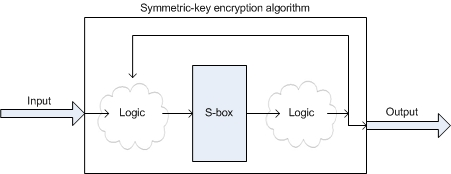
\includegraphics[scale = 0.6]{images/sub_layer.jpg}
\end{figure}
\end{frame}

\begin{frame}
	\frametitle{S-box design}
	Which S-box configurations yield the highest measures of diffusion and confusion?
\end{frame}

\section{Security Measurements}
\begin{frame}
	\frametitle{Security Measurements}
	\begin{itemize}
		\item Branch number 
		\begin{itemize}
			\item Measures lower bound on susceptibility to differential cryptanalysis
		\end{itemize}
		\item Avalanche number
		\begin{itemize}
			\item Measures the total number of bit changes for a single bit change in the input to the S-box
		\end{itemize}
		\item Nonlinearity degree 
		\begin{itemize}
			\item Measures how much nonlinear "behavior" the S-box exhibits by counting the number of output elements that are directly proportional to its input.
		\end{itemize}
	\end{itemize}
\end{frame}

\begin{comment}
\begin{frame}
	\frametitle{Avalanche effect}
A function $f : \field{F}_2^n \to \field{F}_2^n$ exhibits the \emph{avalanche effect} if and only if 
	\begin{eqnarray*}
		\sum_{x \in \field{F}_2^n} \text{wt}(f(x) \oplus f(x \oplus c_{i}^{n})) = n2^{n-1},*
	\end{eqnarray*}
	for all $i (1 \leq i \leq n)$, where $c_{i}^{n} = [0, 0, ..., 1, ..., 0]$ (where a $1$ is in the $n$th position of the vector of cardinality $n$). \\
	%\vspace{0.25cm}
	%This is a significantly stronger sufficient condition for high measures of diffusion.\\
	\vspace{0.25cm}
	*\emph{wt} indicates the Hamming Weight function
\end{frame}

\begin{frame}
	\frametitle{Branch number}
	The \emph{branch number} of an $n \times n$-bit S-Box is
	\begin{eqnarray*}
		BN = \text{min}_{a, b\not=a}(\text{wt}(a \oplus b) + \text{wt}(S(a) \oplus S(b))),
	\end{eqnarray*}
	where $a, b \in \field{F}_2^n$.
\end{frame}

\begin{frame}
	\frametitle{S-box specific nonlinear measurements}
	The nonlinearity of an $n \times n$-bit S-Box from $\field{F}_2^n \to \field{F}_2^n$ can be measured by
	\begin{eqnarray*}
		P_S = \text{max}_{0 \not= a, b}|\{x \in \field{F}_2^n : S(x + a) - S(x) = b\}|
	\end{eqnarray*}
	where $a, b \in \field{F}_2^n$.
\end{frame}
\end{comment}

\begin{frame}
	\frametitle{Known optimal values}
\begin{table}
    \begin{tabular}{|l|l|}
        \hline
        \textbf{Security Measurement} & \textbf{Theoretical Optimal Value} \\ \hline
        Branch number ($B_N$) & $n$ \\ 
        Avalanche number ($A_N$) & $n^22^{n-1}$ \\ 
        Nonlinearity degree ($P_S$) & $1^*$ \\
        \hline
    \end{tabular}
\end{table}
*$P_S \leq 2$ indicates that the function is "almost perfectly nonlinear", which is also a good value
\end{frame}

\begin{frame}
	\frametitle{Exhaustive search for $2$-bit S-box}
\begin{figure}
	\centering
	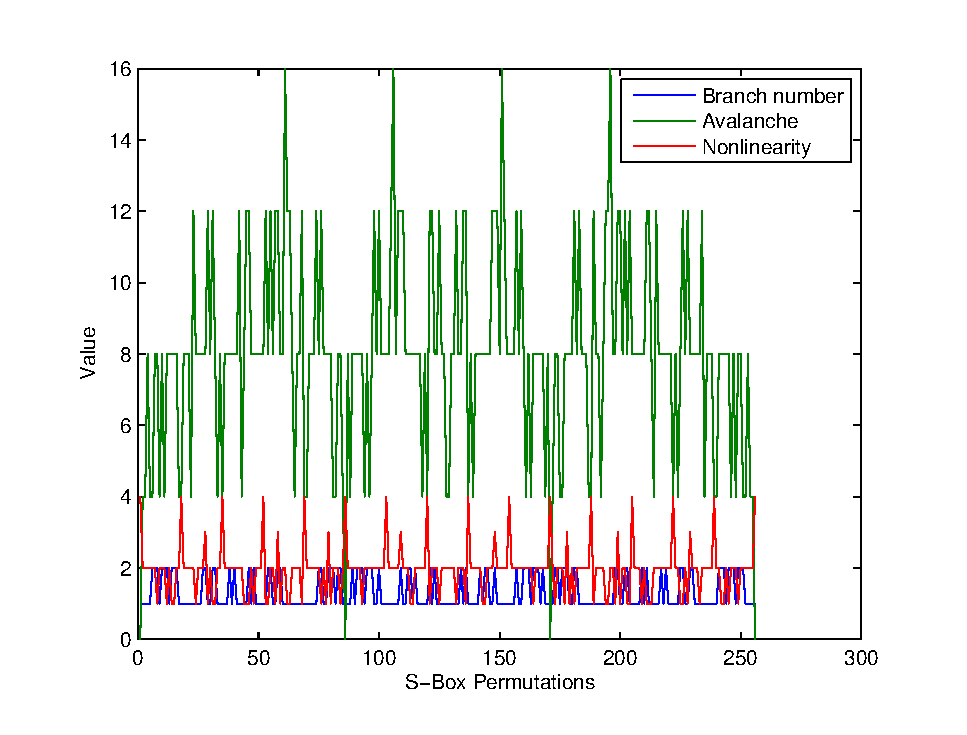
\includegraphics[scale=0.5]{images/brute_joint.eps} 
\end{figure}
\end{frame}

\section{Optimization Problem Formulation}
\begin{frame}
	\frametitle{Branch number problem formulation}
\begin{figure}
\centering
\shadowbox{%
\parbox{11cm}{% 
\textbf{Branch Number - Minimize}
\begin{eqnarray*}
B_N'(X) = -B_N(X) = -\text{min}_{i, j\not=i}(\text{wt}(i \oplus j) + \text{wt}(X(i) \oplus X(j))),
\end{eqnarray*}
subject to the constraints
\begin{eqnarray*}
0 \leq X(i) & \leq & 2^{n} - 1 
\end{eqnarray*}
where $n$ is the number of bits needed to represent the design variables.
}}
\end{figure}
\end{frame}

\begin{frame}
	\frametitle{Avalanche number problem formulation}
\begin{figure}
\centering
\shadowbox{%
\parbox{11cm}{% 
\textbf{Avalanche Number - Minimize}
\begin{eqnarray*}
A_N'(X) = -A_N(X) = -\sum_{i = 0}^{n - 1}\sum_{x \in \field{F}_2^n} \text{wt}(f(x) \oplus f(x \oplus 2^{i}))
\end{eqnarray*}
subject to the constraints
\begin{eqnarray*}
0 \leq X(i) & \leq & 2^{n} - 1 \\
\text{min}_{i, j\not=i}(\text{wt}(i \oplus j) + \text{wt}(X(i) \oplus X(j))) - n2^{n-1} & \leq & 0
\end{eqnarray*}
where $n$ is the number of bits needed to represent the design variables. \\
}}
\end{figure}
\end{frame}

\begin{frame}
	\frametitle{Nonlinearity degree problem formulation}
\begin{figure}
\centering
\shadowbox{%
\parbox{11cm}{% 
\textbf{Degree of Nonlinearity - Minimize}
\begin{eqnarray*}
P_S(X) = \text{max}_{0 \not= a, b}|\{x \in \field{F}_2^n : S(x + a) - S(x) = b\}|,
\end{eqnarray*}
subject to the constraints
\begin{eqnarray*}
0 \leq X(i) \leq 2^{n} - 1,
\end{eqnarray*}
where $n$ is the number of bits needed to represent the design variables. \\
}}
\end{figure}
\end{frame}

\begin{frame}
	\frametitle{Finding a shared solution}
	\begin{itemize}
		\item Create a linear combination of each objective function 
		\item Assign variable weights that correspond to the overall influence of each objective function
	\end{itemize}
\begin{eqnarray*}
f(X) = w_1A_N'(X) + w_2B_N'(X) + w_3P_S(X)
\end{eqnarray*}
\end{frame}
	

\begin{comment}
\begin{figure}
\centering
\shadowbox{%
\parbox{11cm}{% 
\textbf{Joint MINLP Problem - Minimize}
\begin{eqnarray*}
f(X) = w_1A_N'(X) + w_2B_N'(X) + w_3P_S(X),
\end{eqnarray*}
subject to the constraints
\begin{eqnarray*}
0 \leq X(i) & \leq & 2^{n} - 1 \\
\text{min}_{i, j\not=i}(\text{wt}(i \oplus j) + \text{wt}(X(i) \oplus X(j))) - n2^{n-1} & \leq & 0,
\end{eqnarray*}
where $n$ is the number of bits needed to represent the design variables and $w_i$, where $1 \leq i \leq 3$, are \emph{not} design variables. \\
}}
\end{figure}
\end{comment}

\section{Optimization Solution}
\begin{frame}
	\frametitle{MINLP algorithms}
	\begin{itemize}
		\item Traditional MINLP methods
		\begin{itemize}
			\item Branch and Bound (and all derivative) algorithms
		\end{itemize}
		\item Evolutionary methods
		\begin{itemize}
			\item \emph{Genetic algorithm optimization}
			%\item Ant colony optimization
		\end{itemize}
	\end{itemize}
\end{frame}

\begin{comment}
\begin{frame}
	\frametitle{Genetic algorithm configuration}
\begin{table}
	\centering
    \begin{tabular}{|l|l|}
        \hline
        \textbf{Algorithm Option} & \textbf{Configuration Description} \\ \hline
        Population mutation function & Randomly scaled children generations \\ 
        Generations & $500$ \\ 
        Tolerance Function limit & $1 \times 10^{-6}$ from last function value change \\ 
        Stall generation limit & $2^{n^n}$ identical function values \\ 
        Initial population & S-box configuration $\langle 0, 1, ..., n \rangle$ \\
        \hline
    \end{tabular}
	\label{configTable}
\end{table}
\end{frame}
\end{comment}

\begin{frame}
	\frametitle{Avalanche number for $4$-bit S-box}
\begin{figure}
\centering
	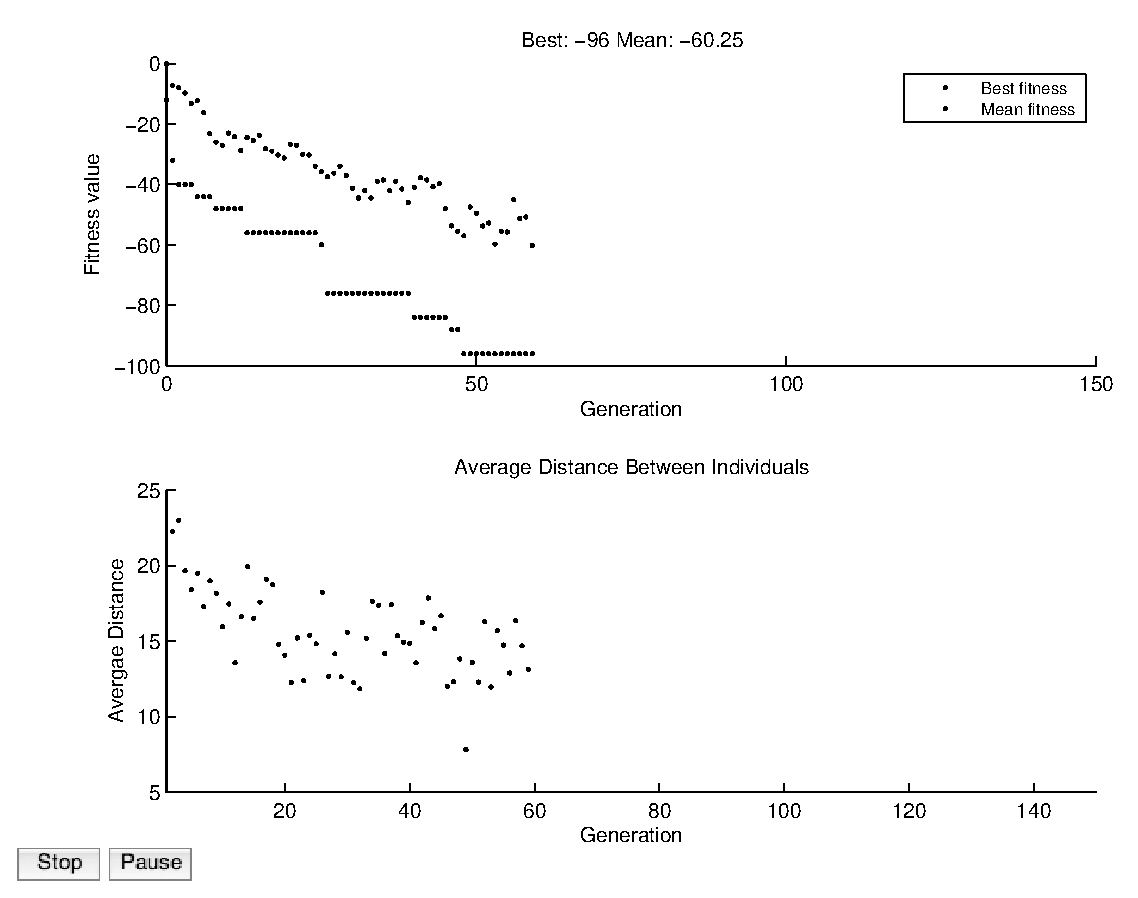
\includegraphics[scale=0.5]{images/avalanche_results16.eps}
\end{figure}
\end{frame}

\begin{frame}
	\frametitle{Branch number for $4$-bit S-box}
\begin{figure}
	\centering
	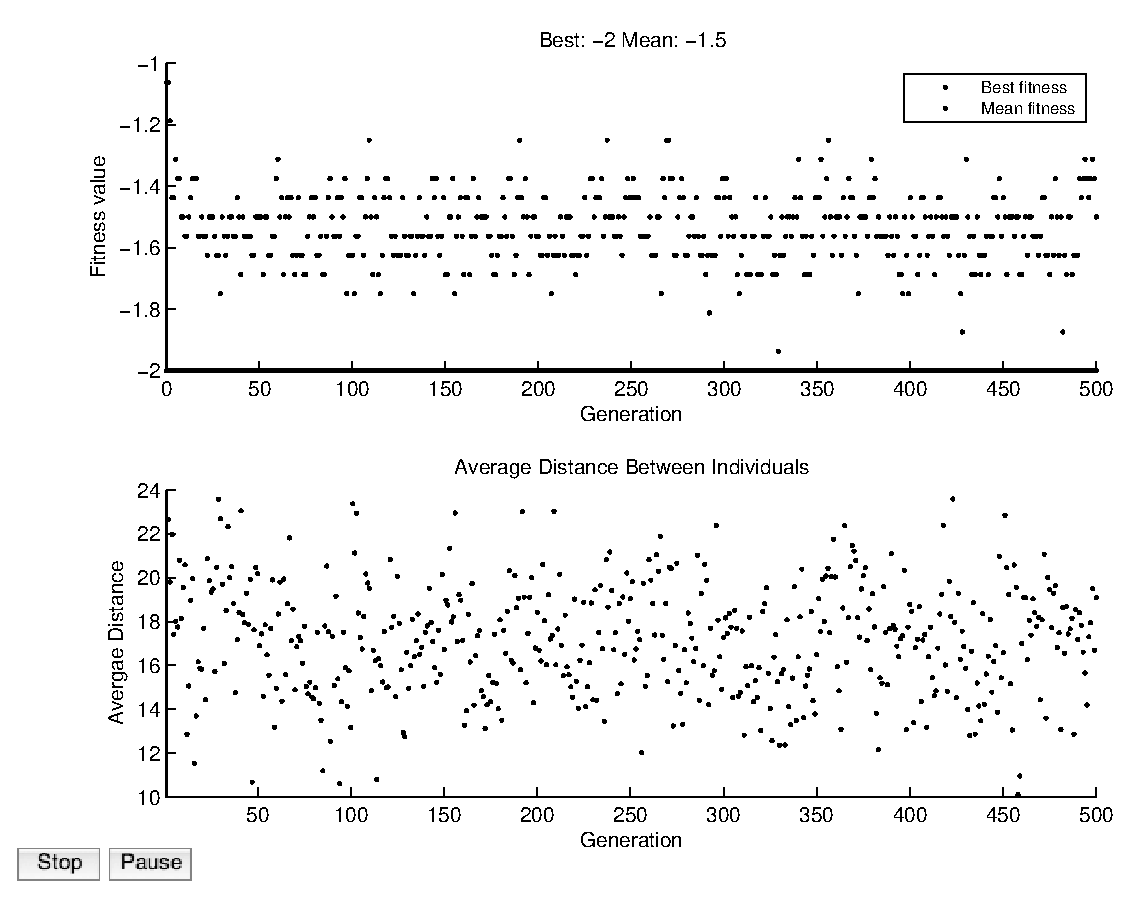
\includegraphics[scale=0.5]{images/bn_results16.eps} 
\end{figure}
\end{frame}

\begin{frame}
	\frametitle{Nonlinearity degree for $4$-bit S-box}
\begin{figure}
	\centering
	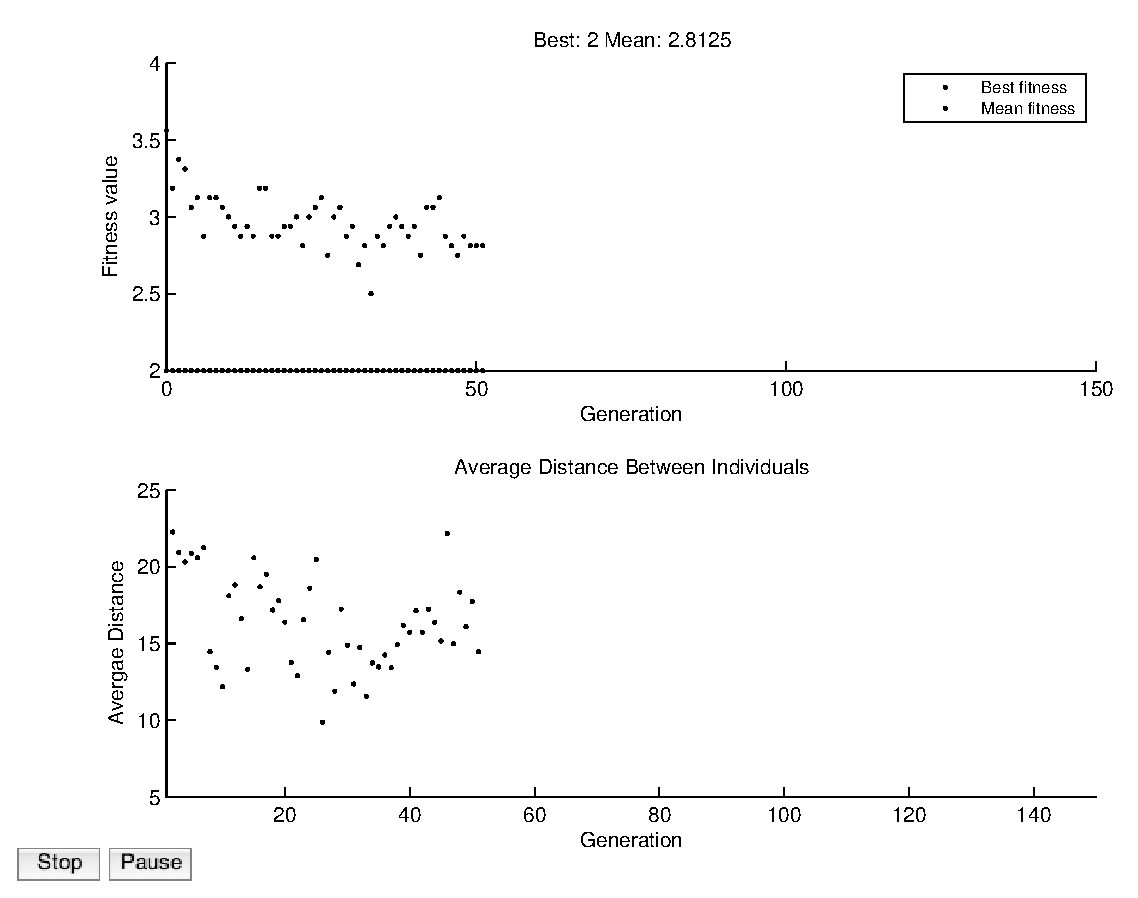
\includegraphics[scale=0.5]{images/nl_results16.eps} 
\end{figure}
\end{frame}

\begin{frame}
	\frametitle{Multi-objective solution for $4$-bit S-box}
\begin{figure}
	\centering
	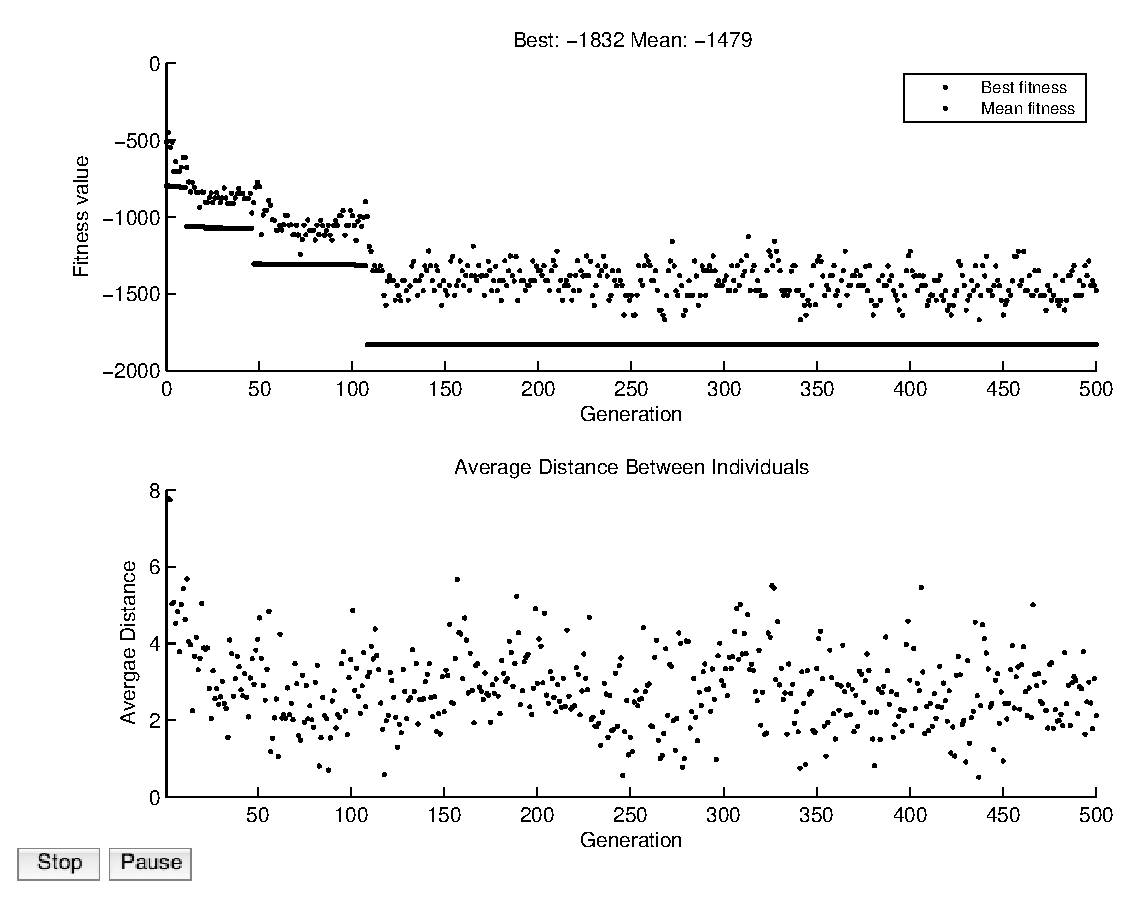
\includegraphics[scale=0.5]{images/joint_results16.eps} 
%	\caption{Weights: $1, 2^8, 2^8$}
\end{figure}
\end{frame}

\section{Final remarks}
\begin{frame}
	\frametitle{Solution Analysis}
\begin{table}
    \begin{tabular}{|l|p{6cm}|}
        \hline
        \textbf{Measurement} & \textbf{Results} \\ \hline
        Branch number & Exponentially less effective with higher order S-boxes \\ 
        Avalanche number & Logarithmically less effective with higher order S-boxes \\ 
        Nonlinearity degree & Consistently effective with all order S-boxes  \\ \hline
	Multi-objective & Ineffective \\
        \hline
    \end{tabular}
\end{table}
\end{frame}

\begin{frame}
	\frametitle{Conclusions}
	\begin{itemize}
		\item Evolutionary optimization algorithms are appropriate for cryptographic applications
		\begin{itemize}
			\item Effectively finds solutions for some discontinuous and instable functions
			\item Not effective at finding solution for multi-objective problems
		\end{itemize}
		\item Difficult to find optimal S-box configurations with high security assurances
		\begin{itemize}
			\item Does not replace hardened proofs of security
		\end{itemize}
	\end{itemize}
\end{frame}

\end{document}
